\subsection{System Overview}
At a core level, the program consists of three or four main modules, the simulation, the renderer, a shared area and the interface, the system is designed using an object orientated structure for the simulation, renderer and shared and makes use of inheritance to reduce code repetition and simplify the underlying structure.

\paragraph{}
The main objects, render and simulation, are run on different threads, this allows the interface to remain responsive even when their is a heavy load on the simulation thread.

\paragraph{}
The shared area inherits the methods in the base class as virtual functions, these consist of set and get functions which will set and return either the control structure or a pointer container, when a pointer container is set, old data is deleted and it creates a copy of the new data to a new pointer. While it is identical, it is a whole new set of data in order to preserve thread-safety. The shared area makes use of polymorphism to modify the functions in the shared area to include mutual exclusion object

\paragraph{}
In order to simplify the management of the bodies objects and remove the automatic out of scope destruction, the objects are allocated using dynamic allocation, the disadvantage of this is that the memory must be kept under check and properly deallocated when it is no longer required. The system that is in place has been verified to delete bodies correctly and does not present any memory leaks.

\paragraph{}
The simulation thread is synchronised to the generally much slower render thread by the use of a condition variable, this interfaces to a mutex object inside the simulation main function and will pause the thread until it is unlocked by a call to the condition variable in the shared area. This effectively locks the iterations to the frame rate one to one unless the iterations per frame is more than 1. While this will result in variance should the frame rate drop below 60 frames per second, this is very unlikely because of how simplistic the graphics are, the simulation will be far slower than the rendering at any body count required to slow down the rendering even on low end and integrated GPUs.

\paragraph{}
The simulation itself makes use of a simplistic brute force method for the simulation. This calculates the forces between every single body in the scenario, this causes the time complexity of the simulation to be $O(n^2)$, the result of this is a dramatic increase in computational complexity with each body added to the simulation. The benefit of this approach is that it is by far the most accurate, as every force is calculated, something like the Barnes-Hut algorithm is less accurate, as it further approximates large clusters of bodies considering them as one large mass in a weighted mean, however this brings more advantages in terms of computation, reducing the time complexity to $O(nlogn)$.

\paragraph{}
In order to improve long term stability and general accuracy of the approximation, leapfrog integration is used, standard euler integration results in a massive deviation from initial system energies due to an accumulation of errors, this results in velocity being calculated at half time steps, while position and acceleration are calculated together. This results in a much greater stability of the simulation in both short term and long term. It also allows for the simulation to be reversed.

\paragraph{}
All forces are calculated directly as acceleration, each relationship calculated adds extra acceleration to the bodies in the $x$ and $y$ components respectively, half period velocity change and position are calculated in individual body objects directly.

\paragraph{}
The render module is relatively basic, containing functions for rendering individual bodies and the whole scene as a whole (Every body). The render class also contains a method for the creation of superstructures, a large collection of bodies all orbiting around a single point.

\paragraph{}
The interface itself is significantly less structured, as the program has to interface several different programming paradigms, including object orientated, standard procedural and event driven programming methodologies in the form of callback functions that must be set at program initialization. GLFW callbacks are passed through to AntTweakBar to allow it to access the input. The GLFW callbacks are also used for control of the camera and selection of bodies. Due to the way these callbacks work (Function Pointers), it is not directly possible to have them part of a class.

\paragraph{}
The GUI for the program was intentionally kept basic, none of the windows link together and they are all managed by the facilities of the AntTweakBar library.

\paragraph{}
Worth noting is that the AntTweakBar library is no longer maintained by the developer, the source for this library required a slight modification in order to work with the newest version of GLFW, namely when it comes to handling of inputs as the names of some decelerations have changed. The binary would need to be recompiled for this library, the modified source would likely be distributed with the source code package for the program itself, the original developer provided build systems for different operating systems so as long as dependencies are satisfied, building the modified library is straightforward. (This is not of concern to the primary user.)

\paragraph{}
Some alternative GUI packages do exist and they are actively developed, however they tend to be a lot more custom and are not as simple to set up. However having better integration into the program and an active developer community for support may outweigh this disadvantage. It would also allow for more comprehensive UI which could be far more usable and easier to add extensions to.
\pagebreak

\subsection{Algorithm Design}
\subsubsection{Calculation of All Acceleration Relationships}
This algorithms was initially extremely complex in the original specification, however after further review, it was realised that the majority of the code that was present was very redundant and only served as a memory hog. Originally the force was calculated, populated into the body objects and then acceleration was calculated on the body objects themselves.

\paragraph{}
The new code is far simpler, for starters, the force is no longer stored on the body objects, instead the force is calculated for the relationship and then it is converted to acceleration and applied to both bodies in the same method, because acceleration is still a vector quantity it can be added up in the same way that force is.

\paragraph{}
Boiling it down, this algorithm is simply a double for loop, however it makes use of the outer for loop to offset the inner for loop, effectively 'cutting-off' one half of a 'matrix'. (Including the central diagonal.) The benefit of this method is that there is no requirement to store the force in an actual matrix array, which saves on a large amount of memory. (Memory usage of a 2D array is $n^2$, which is excessive.)

\paragraph{}
The outer and inner variables are used to iterate through the body storage container, which contains pointers to the body objects. These pointers are passed to the single pair calculation method which populates both of the bodies with the acceleration produced by that relationship. Going through the double for loop will populate all of the bodies in the scenario with forces created by every other body.

\paragraph{Pseudocode}
\begin{algorithmic}[1]
\FOR{$Body_A \leftarrow 1$ \TO Bodies} 
  \FOR{$Body_B \leftarrow (Body_A+1)$ \TO Bodies}
    \STATE $Acceleration(Body_A,Body_B)$
  \ENDFOR
\ENDFOR
\end{algorithmic}

\paragraph{}
For 5 bodies, This produces iteration in order. \\
$0-1$, $0-2$, $0-3$, $0-4$, $1-2$, $1-3$, $1-4$, $2-3$, $2-4$, $3-4$ \\
No extra conditionals are required to check that $x \neq y$, Improving performance.

\pagebreak

The following is code for the above algorithm and for calculation of single relationships.
\begin{lstlisting}[language=c++]
  void simulation::calcAcceleration(body* bA, body* bB) {
    // Calculate and store distances for calculation
    double dX = getComponentDistance(bA, bB, 0);
    double dY = getComponentDistance(bA, bB, 1);
    double dV = getVectorDistance(dX, dY);

    // F=GmM/(r^3) - Pre-component force
    double fP = -(lControl.UGC * bA->m * bB->m) / std::pow(dV,3);
    // Component Forces
    double fX = fP * dX;
    double fY = fP * dY;

    // a=F/m - Set acceleration to bodies
    // Body A
    bA->aX +=  fX / bA->m;
    bA->aY +=  fY / bA->m;
    // Body B
    bB->aX += -fX / bB->m;
    bB->aY += -fY / bB->m;
  }   
  
  void simulation::calcAllAcceleration(void) {
  resetAllAcceleration(); // Set all accelerations to 0;
    for(unsigned int x = 0; x < bodies.size(); x++) {
      // Evaluate bottom left of calculation matrix
      for(unsigned int y = x+1; y < bodies.size(); y++) {
        // Same body relationships do not occur
        calcAcceleration(bodies[x], bodies[y]);
      }
    } 
  }
\end{lstlisting}

\subsubsection{Leapfrog Integration}
Leapfrog integration is the core to the stability and time-realisability functionality of the simulation. At a basic level, leapfrog integration in simply a rearrangement of the order in which Acceleration, Velocity and Position are calculated.

\paragraph{}
The euler approach is what the majority of basic physics problems will end up using, generally because they are only asking for a single 'iteration' in order to find a solution.

\subsubsection{Mutex Locks on Shared Data}

\subsubsection{Calculate Collisions}

\subsubsection{Creation of Superstructure}

\subsubsection{Update UI / Update Body}

\begin{sidewaysfigure}
\subsection{Function Listing}
  \subsubsection{Main}
  \centering  
  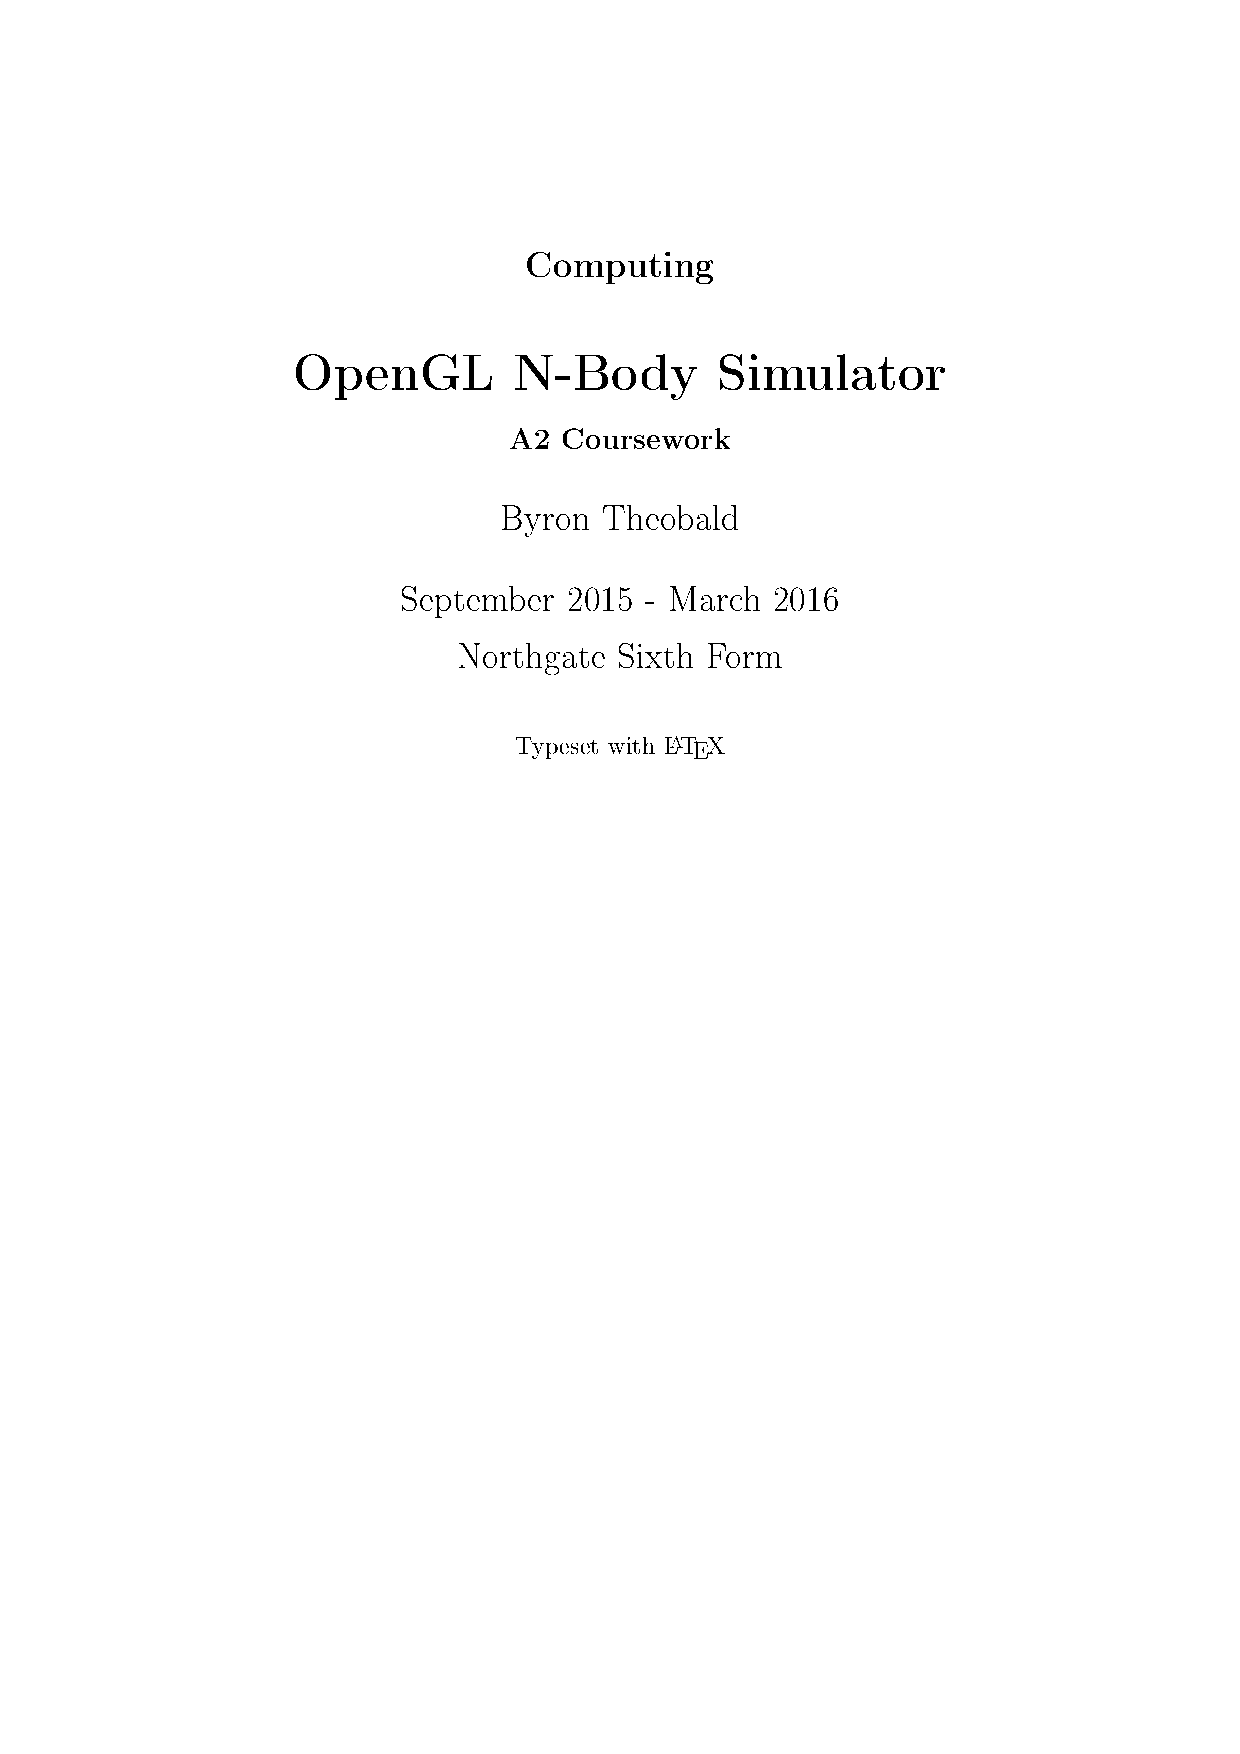
\includegraphics[width=\textwidth]{img/functions/main.png}
\end{sidewaysfigure}

\begin{sidewaysfigure}
  \subsubsection{Body}
  \centering  
  \includegraphics[width=\textwidth]{img/functions/body.png}
\end{sidewaysfigure}

\begin{sidewaysfigure}
  \subsubsection{Scenario}
  \centering  
  \includegraphics[width=\textwidth]{img/functions/scenario.png}
\end{sidewaysfigure}

\begin{sidewaysfigure}
  \subsubsection{Render}
  \centering  
  \includegraphics[width=\textwidth]{img/functions/render.png}
\end{sidewaysfigure}

\begin{sidewaysfigure}
  \subsubsection{Simulation}
  \centering  
  \includegraphics[width=\textwidth]{img/functions/simulation.png}
\end{sidewaysfigure}

\begin{sidewaysfigure}
  \subsubsection{Shared}
  \centering  
  \includegraphics[width=\textwidth]{img/functions/shared.png}
\end{sidewaysfigure}

\begin{sidewaysfigure}
  \subsubsection{UI}
  \centering  
  \includegraphics[width=\textwidth]{img/functions/ui.png}
\end{sidewaysfigure}

\begin{sidewaysfigure}
  \centering  
  \includegraphics[width=\textwidth]{img/functions/ui2.png}
\end{sidewaysfigure}

\subsection{Variable Listing}
\begin{figure}[H]
   \centering
   \includegraphics[page=1, width=\textwidth]{../varlist.pdf} 
\end{figure}

\begin{figure}[H]
   \centering
   \includegraphics[page=2, width=\textwidth]{../varlist.pdf} 
\end{figure}

\begin{figure}[H]
   \centering
   \includegraphics[page=3, width=\textwidth]{../varlist.pdf} 
\end{figure}